\documentclass[12pt]{article}

\usepackage[top=50pt, bottom=50pt, left=90pt, right=90pt]{geometry}
\usepackage[pdftex]{graphicx}
\usepackage{soul}

\usepackage{lipsum}%% a garbage package you don't need except to create examples.
\usepackage{fancyhdr}
\pagestyle{fancy}

%This is some header and footer information
\lfoot{Kids Coding Club}
\rfoot{\thepage}
\cfoot{}
\renewcommand{\headrulewidth}{0pt}
\renewcommand{\footrulewidth}{0.4pt}

%Basic title information about original author and title
\title{Class 5 - Arduino and Motors}
\author{Chris Hight}
\date{\today}
 

\begin{document}

\maketitle


\section *{Introduction to the Project}
	\begin{itemize}
		\item During this project we are going to setup two motors and activate them using a sonic sensor to judge distance to an object

		\item The parts we are going to use are:
	
		\begin{itemize}
    		\item Arduino - This is our bots "brain"
    		\item Breadboard - This is how we can connect arduino and parts together
    		\item Motors - These will turn our wheels
    		\item H-Bridge Motor Driver - This is a chip that helps control our motors
    		\item Ultrasonic Sensor - This tells distance like a dolphin does, it sends out a really high pitch noise and waits for it to come back
		\end{itemize}
		
		\item In the second hour you will need to use the ultrasonic sensor to make your robot move, you will learn how to do that in this lesson
	
	\end{itemize}



\section *{Let's Connect Our Motors}
	\begin{itemize}
		\item We are going to start with three parts, arduino, breadboard and h-bridge motor driver. 
		\begin{center}
    		\begin{figure}[h!]
				\begin{minipage}[t]{0.48\textwidth}
					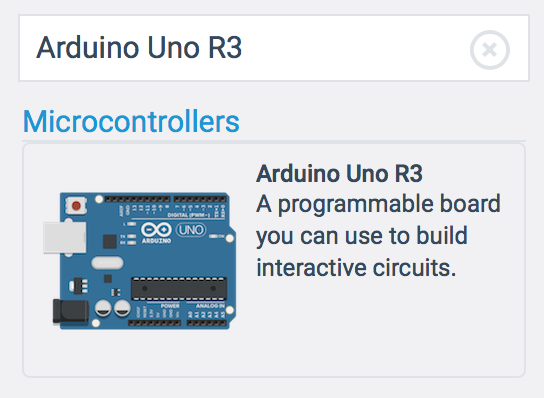
\includegraphics[scale = 0.71]{./Images/arduino}
				\end{minipage}
				\hspace*{\fill} % it's important not to leave blank lines before and after this command
				\begin{minipage}[t]{0.48\textwidth}
					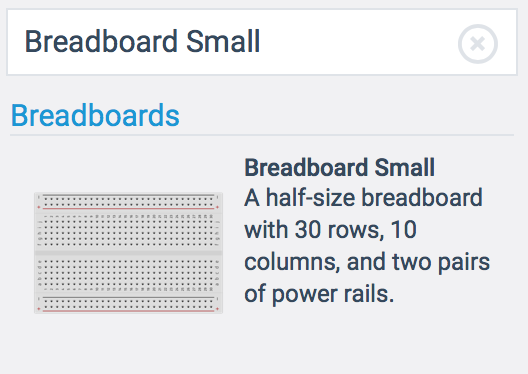
\includegraphics[scale = 0.75]{./Images/breadboard}
				\end{minipage}
			\end{figure}
			\item H-Bridge Motor Driver will attach to our breadboard
			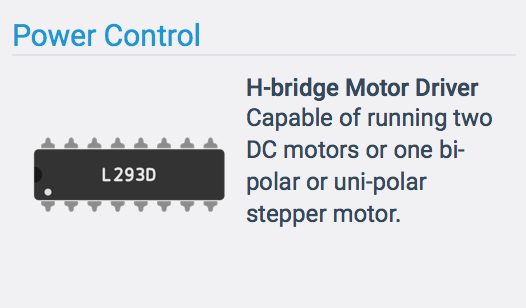
\includegraphics[scale = 0.75]{./Images/hmotor}
		\end{center}
		
		\item Laying out the parts should look something like this:
		\begin{center}
			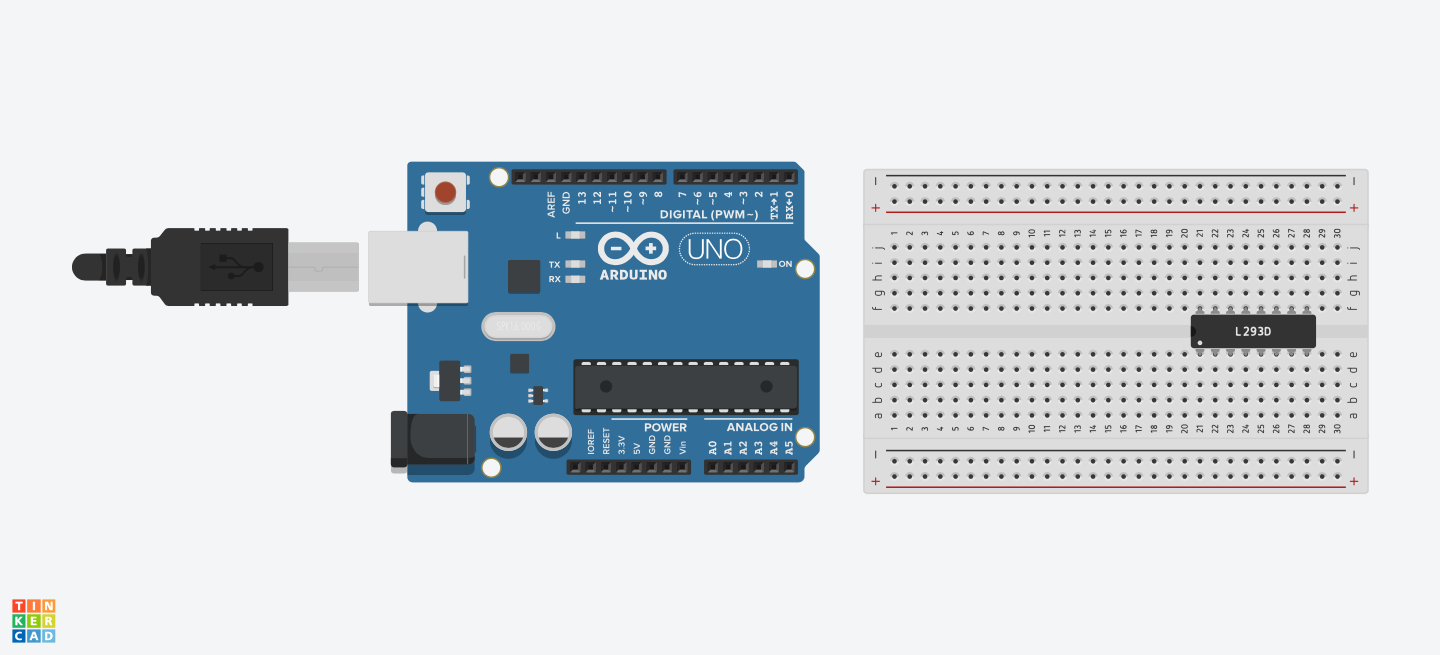
\includegraphics[scale = 0.3]{./Images/circuit1}
		\end{center}
		\item Next we are going to want to hook up the Power to our circuit
			\begin{itemize}
				\item For power we tend to use red wire for positive and black wire for negative
				\item Explain: VCC and 5V are the same as positive.  Ground is the same as negative
			\end{itemize}
		\begin{center}
			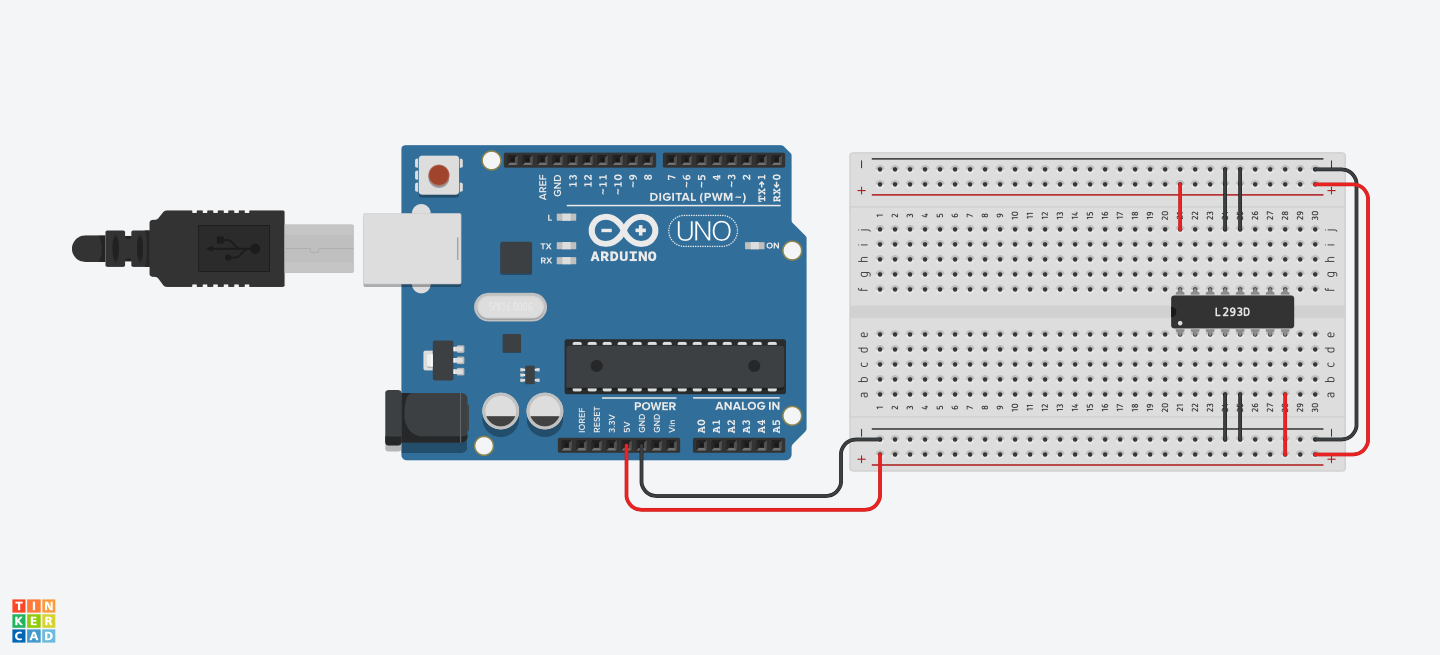
\includegraphics[scale = 0.3]{./Images/circuit2}
		\end{center}
		\item Now we need to bring in two different motors and place them on either side of the breadboard.  
		\begin{center}
			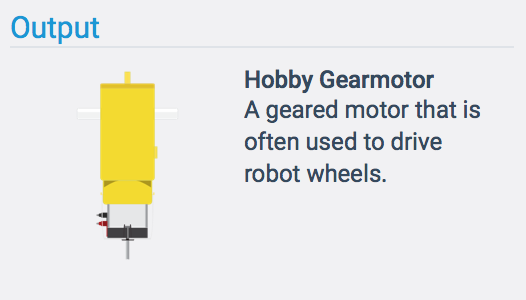
\includegraphics[scale = 0.7]{./Images/motor}
		\end{center}
		\item We are going to connect our motors to the chip on the breadboard. This chip translates what we tell it to do and makes the motors actually do it  
		\item Let's add the motors:
		\begin{center}
			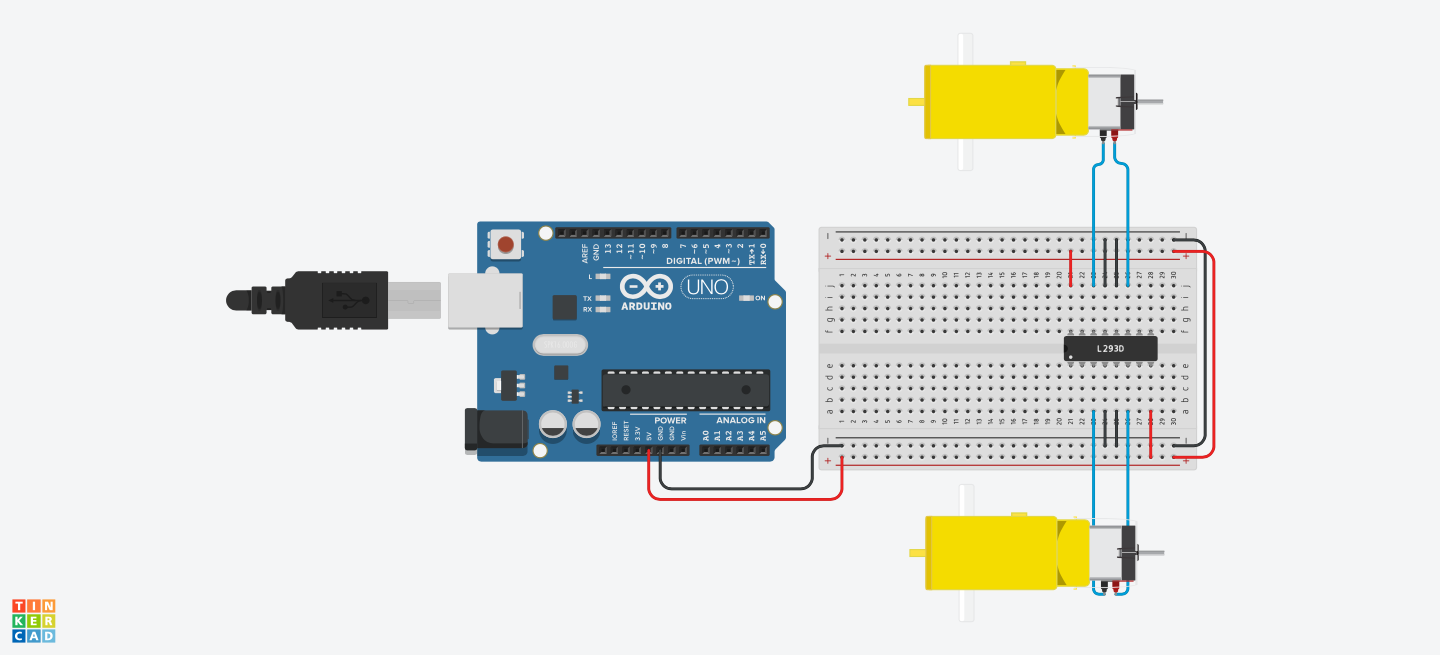
\includegraphics[scale = 0.3]{./Images/circuit3}
		\end{center}
		\item Now we have connected the output but we have no input.  We give the chip power but that isn't enough to tell the motors to turn. 
		\newpage
		\item We are going to hook the chip up to the arduino \textbf{First Motor}:
		\begin{center}
			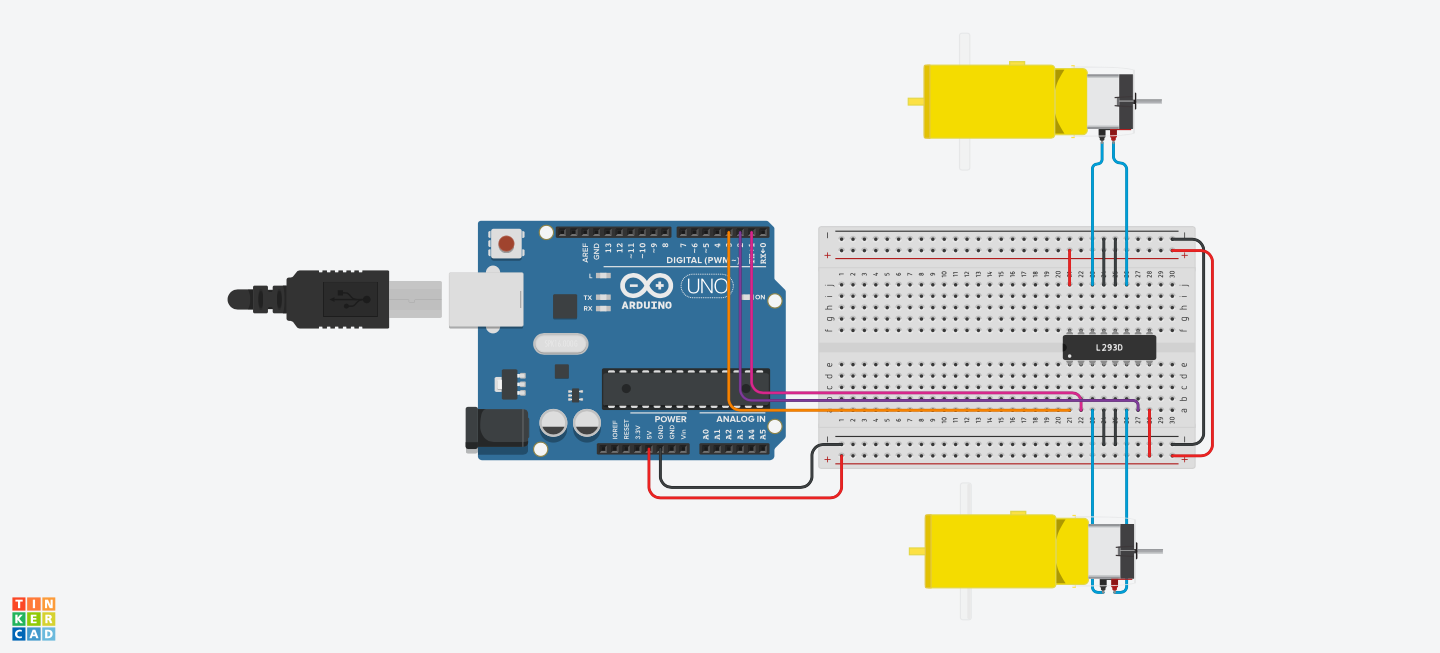
\includegraphics[scale = 0.3]{./Images/circuit4}
		\end{center}
		\item Each side of the chip controls one motor.
		\item Now lets hook up the other side of the chip \textbf{Second Motor}
		\begin{center}
			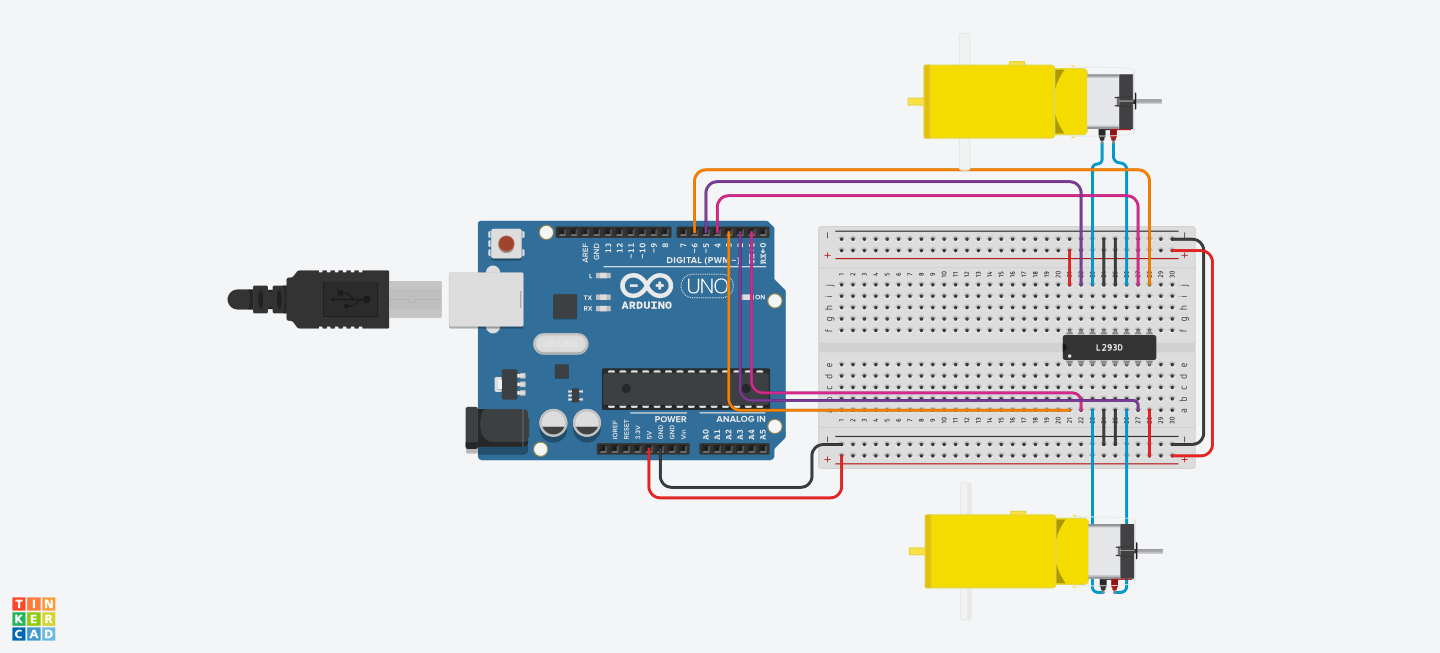
\includegraphics[scale = 0.3]{./Images/circuit5}
		\end{center}
	\end{itemize}







 
\section *{Coding Motor Movement}
	\begin{itemize}
		\item There are three pins that control our motor chip. 
		\begin{itemize}
			\item 1 pin controls the speed, a value of 0 makes it turn at 0 percent, a value of 255 makes it turn at 100 percent.
			\item The two other pins do the same thing but work opposite of each other.  If we want it to turn clockwise we will turn the first pin off and second pin on, to go counterclockwise we do just the opposite, first pin on and second pin off.
		\end{itemize}
		\item To make the first motor move use the code below:
		\begin{center}
			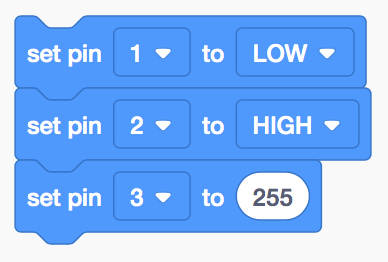
\includegraphics[scale = 0.7]{./Images/code1}
		\end{center}
		\item What happens if we set pin 3 to 300 instead of 255?  Will it run faster or slower.
		\item Let's make the second motor move now using the code:
		\begin{center}
			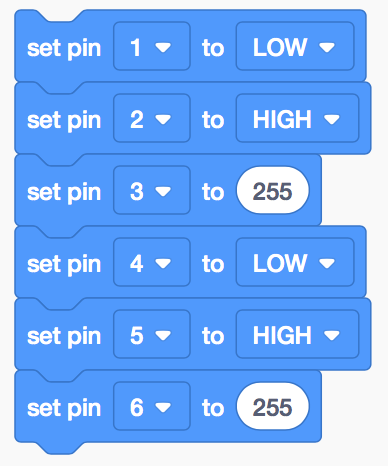
\includegraphics[scale = 0.7]{./Images/code2}
		\end{center}
	\end{itemize}
	
	
	
	
	
	
	
	
	
	
	
	
\section *{Wire in the Ultrasonic Motor}
	\begin{itemize}
		\item We need to search for the Ultrasonic sensor and add that above the arduino board.
		\begin{center}
			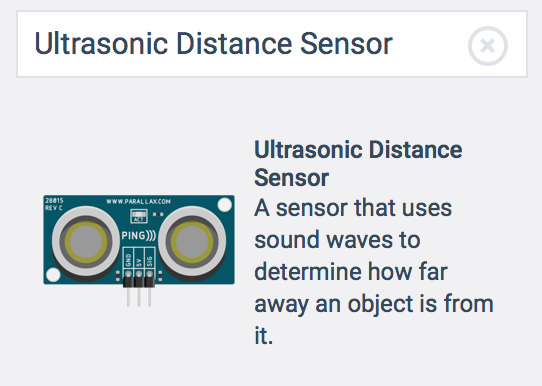
\includegraphics[scale = 0.7]{./Images/ultrasonic}
		\end{center}
		\item We will wire the power to the Ultrasonic sensor.  
		\newpage
		\item After that we need to input the signal lead into a spot on the Arduino, we can use pin 9.
		\begin{center}
			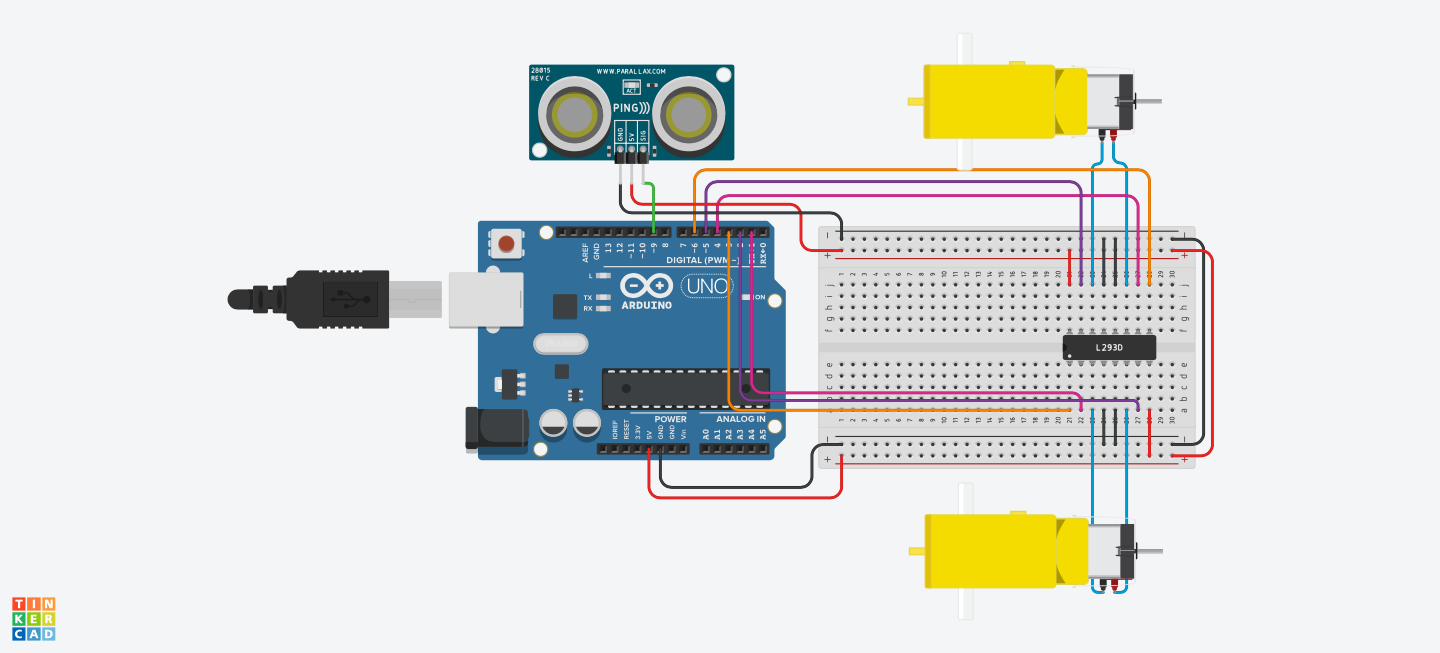
\includegraphics[scale = 0.3]{./Images/circuit6}
		\end{center}
	\end{itemize}
	
	
	
	
	
	
\section *{Write Code to Use Ultrasonic Sensor}
	\begin{itemize}
		\item Using the Input blocks there is a block that allows us to read the distance using an Ultrasonic sensor.
		\item We set this inside of an operator blow allowing us to check if the ultrasonic sensor is ever above a specific number, let's use \textbf{45}
		\item We want to know when this is true and when it is then we want to move the motors.  Use an \textbf{if then else} block. 
		\item Put the code together to look like this:
		\begin{center}
			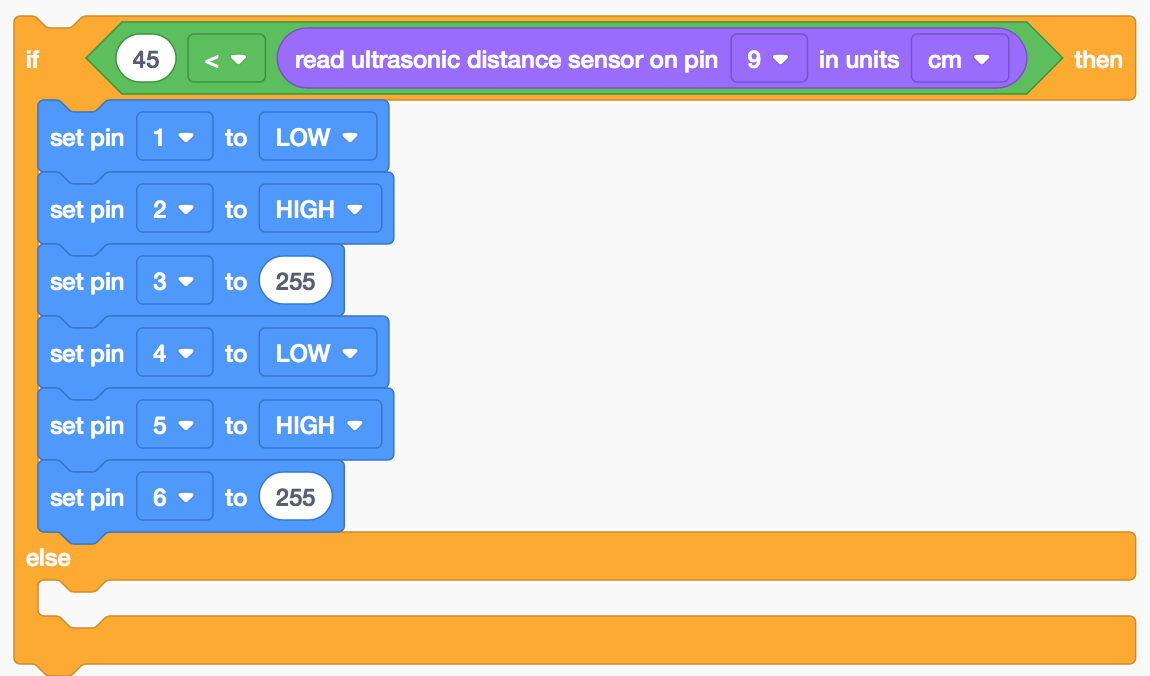
\includegraphics[scale = 0.7]{./Images/code3}
		\end{center}
		\item \textbf{Why do we need the else?} This will be where we turn the motors off.
		\item In the else we need to set pin 6 and 3 to 0.  This will stop the motor rotation
		\begin{center}
			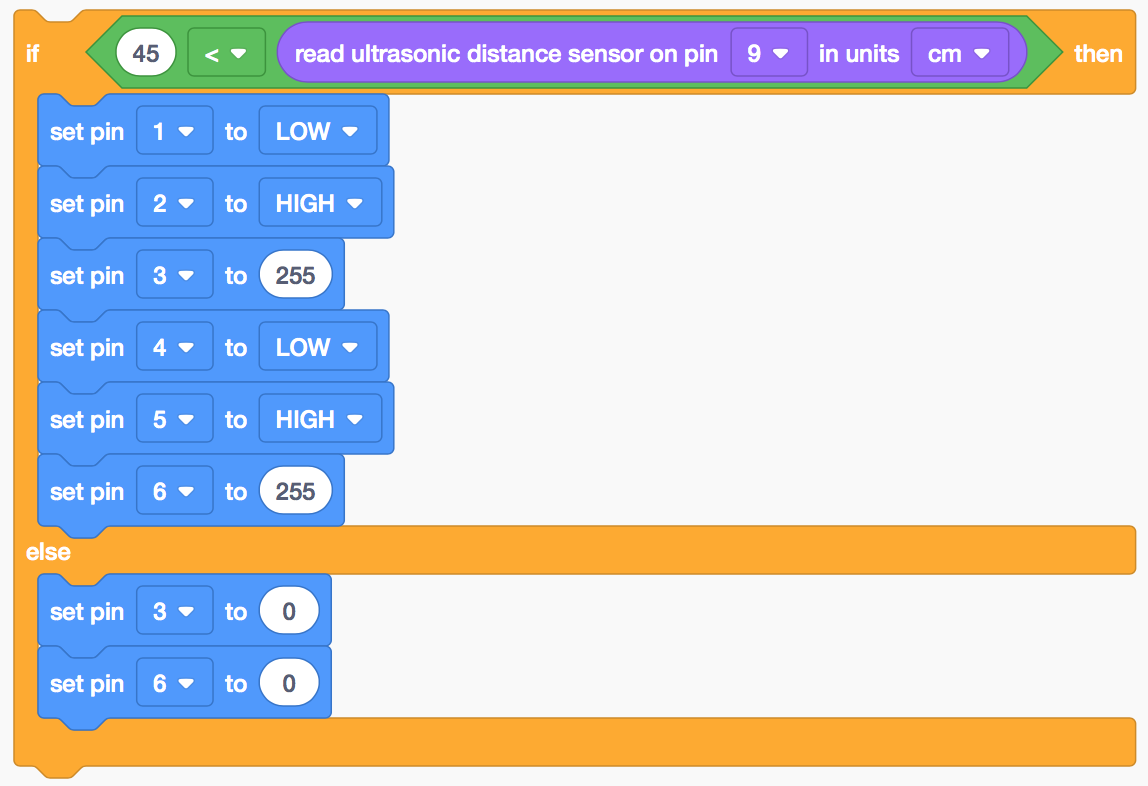
\includegraphics[scale = 0.6]{./Images/code4}
		\end{center}
		\item We want this to check forever, right?  Well we don't have a forever loop here but we can make one.
		\item We will use a \textbf{repeat while} loop and inside of it we will use an operation that will compare 1 = 1.  Since 1 is always equal to 1 in a repeat loop it will always be true.
		\begin{center}
			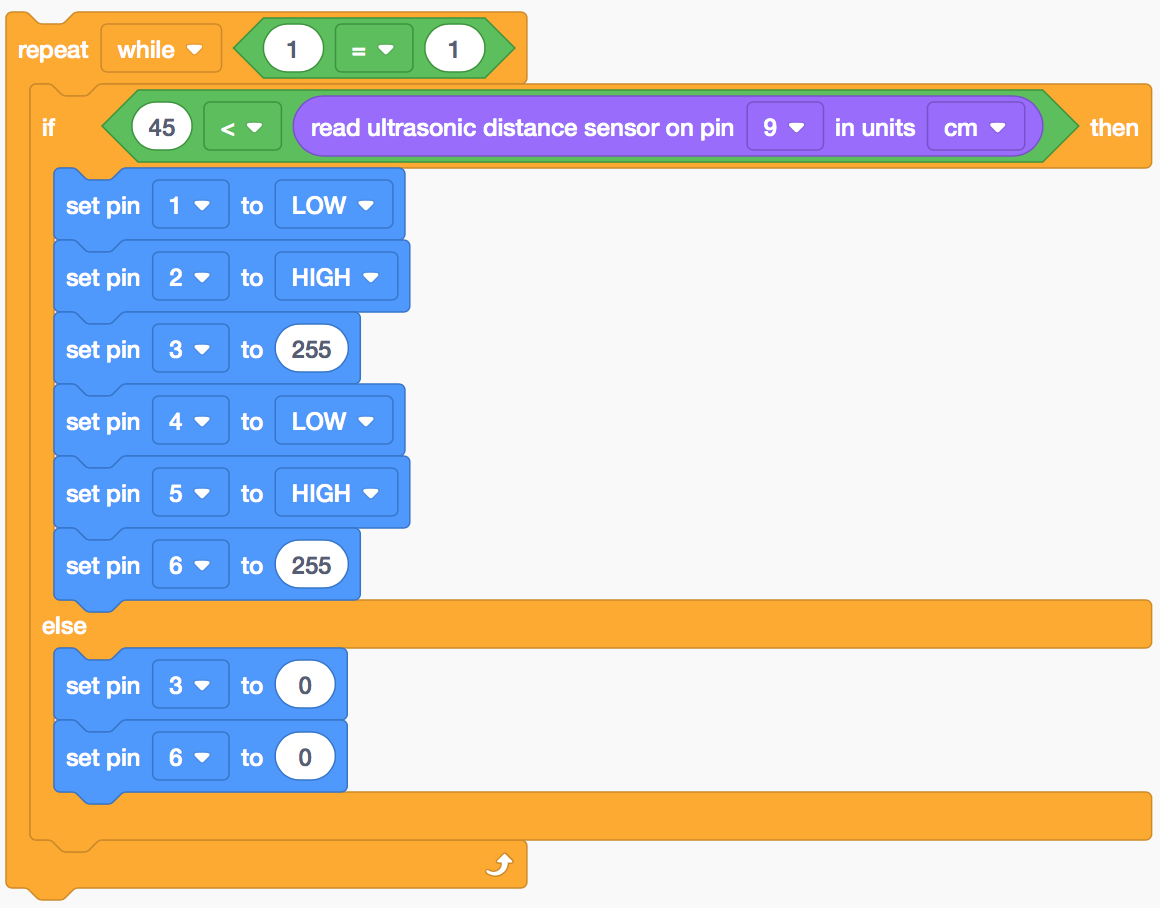
\includegraphics[scale = 0.6]{./Images/code5}
		\end{center}
		\item Now, test it!
	\end{itemize}
	
\end{document}
